\documentclass[border=8pt]{standalone}
\usepackage{tikz}
\usetikzlibrary{arrows.meta,positioning,calc}
\begin{document}
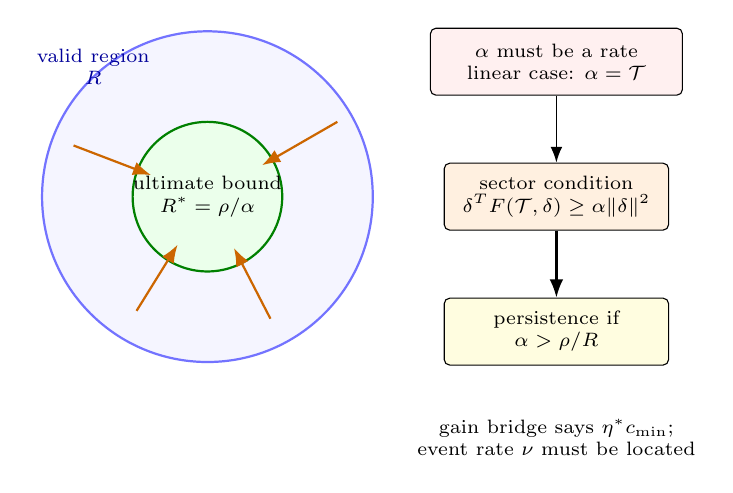
\begin{tikzpicture}[
  box/.style={draw, rounded corners=2pt, align=center, minimum width=2.85cm, minimum height=0.85cm, font=\scriptsize},
  note/.style={align=center, font=\scriptsize},
  arr/.style={-Latex, thick},
  thinarr/.style={-Latex, semithick}
]

\coordinate (o) at (0,0);
\draw[fill=blue!4, draw=blue!55, thick] (o) circle (2.1cm);
\draw[fill=green!8, draw=green!50!black, thick] (o) circle (0.95cm);
\node[note] at (0,0) {ultimate bound\\$R^\ast=\rho/\alpha$};
\node[note, blue!60!black] at (-1.45,1.65) {valid region\\$R$};

\foreach \x/\y in {1.65/0.95, -1.7/0.65, 0.8/-1.55, -0.9/-1.45} {
  \draw[arr, orange!80!black] (\x,\y) -- ($(o)!0.42!(\x,\y)$);
}

\node[box, fill=orange!12, right=3.0cm of o] (sector)
  {sector condition\\$\delta^T F(\mathcal T,\delta)\geq\alpha\|\delta\|^2$};
\node[box, fill=yellow!12, below=0.85cm of sector] (persist)
  {persistence if\\$\alpha>\rho/R$};
\draw[arr] (sector) -- (persist);

\node[box, fill=red!6, above=0.85cm of sector, minimum width=3.2cm] (rate)
  {$\alpha$ must be a rate\\linear case: $\alpha=\mathcal T$};
\draw[thinarr] (rate) -- (sector);

\node[note, below=0.55cm of persist] {gain bridge says $\eta^\ast c_{\min}$;\\event rate $\nu$ must be located};

\end{tikzpicture}
\end{document}
